\documentclass[UTF8,12pt, a4paper]{ctexart}
\usepackage{geometry}
\usepackage{listings}
\usepackage{xcolor}
\usepackage{amsmath}
\usepackage{graphicx}
\usepackage{rotating}
\usepackage{arydshln}

\geometry{left=2.0cm, right=2.0cm, top=1.0cm, bottom=2.5cm}

  \title{矩阵分析作业6:模和内积}
  \author{ 2019.11.01}
  \date{}
  \begin{document}
  \maketitle
  \pagestyle{plain}
  \allowdisplaybreaks

  \subsection*{Exercise.3}
  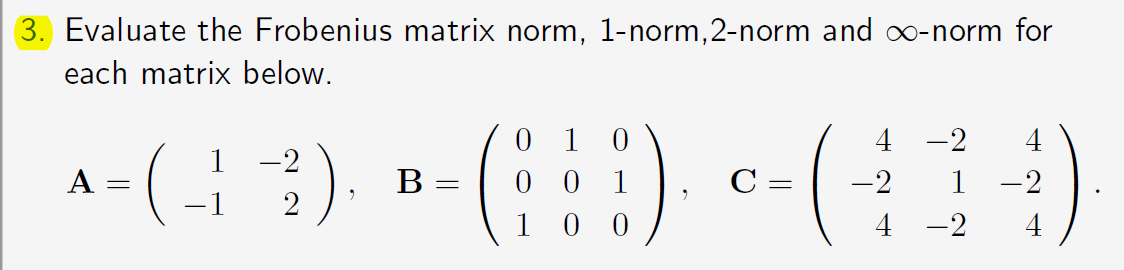
\includegraphics[scale=0.8]{question3.png} \\
  (1).对于矩阵A,首先计算$A^*A$的特征值,
  $$
  \begin{aligned}
    A^*A-\lambda I = 
    \left(
      \begin{matrix}
        &2-\lambda & -4 \\
        & -4 & 8-\lambda
      \end{matrix}
    \right)
  \end{aligned}
  $$

  由$(2-\lambda)(8-\lambda)-16=0$可得$\lambda_1=10,\ \lambda_2 = 0$,因此可得,
  $$
  \begin{aligned}
    ||A||_2 &= \sqrt{\lambda_{max}} = \sqrt{10} \\
    ||A||_F &= \left(\sum_{i,j}{|a_{ij}^2|}\right)^{\frac{1}{2}} = \sqrt{10}\\
    ||A||_1 &= \mathop{max} \limits_{j}\sum_{i}{|a_{ij}|} = 4 \\
    ||A||_{\infty} &= \mathop{max} \limits_{i}\sum_{j}{|a_{ij}|} = 3 \\
  \end{aligned}
  $$
  (2).对于矩阵B,首先计算$B^*B$的特征值,
  $$
  \begin{aligned}
    B^*B-\lambda I = 
    \left(
      \begin{matrix}
        &1-\lambda &0 &0 \\
        &0 & 1-\lambda &0 \\
        &0 &0 &1-\lambda
      \end{matrix}
    \right)
  \end{aligned}
  $$

  由$(1-\lambda)^3=0$可得$\lambda=1$,因此可得,
  $$
  \begin{aligned}
    ||B||_2 &= \sqrt{\lambda_{max}} = 1 \\
    ||B||_F &= \left(\sum_{i,j}{|b_{ij}^2|}\right)^{\frac{1}{2}} = \sqrt{3}\\
    ||B||_1 &= \mathop{max} \limits_{j}\sum_{i}{|b_{ij}|} = 1 \\
    ||B||_{\infty} &= \mathop{max} \limits_{i}\sum_{j}{|b_{ij}|} = 1 \\
  \end{aligned}
  $$
  (3).对于矩阵A,首先计算$C^*C$的特征值,
  $$
  \begin{aligned}
    C^*C-\lambda I = 
    \left(
      \begin{matrix}
        &36-\lambda &-18 &36 \\
        &-18 &9-\lambda &-18 \\
        &36 &-18 &36-\lambda
      \end{matrix}
    \right)
  \end{aligned}
  $$

  由$|C^*C-\lambda I| = 0$可得$\lambda _1=81,\ \lambda_2=\lambda_3 = 0$,因此可得,
  $$
  \begin{aligned}
    ||C||_2 &= \sqrt{\lambda_{max}} = \sqrt{81} = 9 \\
    ||C||_F &= \left(\sum_{i,j}{|c_{ij}^2|}\right)^{\frac{1}{2}} = \sqrt{81}=9\\
    ||C||_1 &= \mathop{max} \limits_{j}\sum_{i}{|c_{ij}|} = 10 \\
    ||C||_{\infty} &= \mathop{max} \limits_{i}\sum_{j}{|c_{ij}|} = 10 \\
  \end{aligned}
  $$
  
\subsection*{Exercise.10}
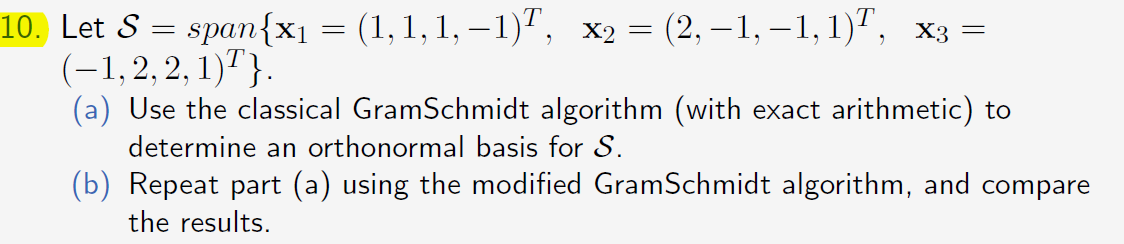
\includegraphics[scale=0.8]{question10.png}\\
(a)施密特正正交化过程如下:
\begin{align*}
  k=1: &\  u_1 \leftarrow \frac{x_1}{||x_1||} 
  = \frac{1}{2}
  \left(
    \begin{matrix}
      1 \\ 1\\ 1\\ -1
    \end{matrix}
  \right) \\
  k=2: &\  u_2 \leftarrow x_2-(u_1^Tx_2)u_1 
  = x_2+\frac{1}{2}u_1 
  = \frac{1}{4} 
  \left(
    \begin{matrix}
      9 \\ -3 \\ -3 \\ 3
    \end{matrix}
  \right),\ u_2\leftarrow \frac{u_2}{||u_2||}
  = \frac{\sqrt{3}}{6} \left(
    \begin{matrix}
      3 \\ -1 \\ -1 \\ 1
    \end{matrix}  
  \right) \\
  k=3: &\  u_3 \leftarrow x_3 -(u_1^T x_3)u_1 - (u_2^Tx_3)u_2 =x_3-u_1+\sqrt{3}u_2 
  =\left(
    \begin{matrix}
      0 \\ 1 \\ 1 \\ 2
    \end{matrix}  
  \right) \\
  &\  u_3 \leftarrow \frac{u_3}{||u_3||} 
  = \frac{1}{\sqrt{6}} \left(
    \begin{matrix}
      0 \\ 1 \\ 1 \\ 2
    \end{matrix}  
  \right)\\
  thus: \\
  &\  u_1=\frac{1}{2}
  \left(
    \begin{matrix}
      1 \\ 1\\ 1\\ -1
    \end{matrix}
  \right),
  u_2=\frac{\sqrt{3}}{6} 
  \left(
    \begin{matrix}
      3 \\ -1 \\ -1 \\ 1
    \end{matrix}  
  \right) ,
  u_3=\frac{1}{\sqrt{6}} 
  \left(
    \begin{matrix}
      0 \\ 1 \\ 1 \\ 2
    \end{matrix}  
  \right)
\end{align*}

所以$\{ u_1,u_2,u_3\}$构成了$\mathcal{S}$空间的一组标准正交基。\\
(b) 使用改进的施密特正交化过程如下:
\begin{align*}
  k=1:\  &u_1 \leftarrow \frac{x_1}{||x_1||} 
  = \frac{1}{2}
  \left(
    \begin{matrix}
      1 \\ 1\\ 1\\ -1
    \end{matrix}
  \right),so
  \{u_1,u_2,u_3\}\leftarrow\{u_1, x_2,x_3\} \\
  k=2:\  & (u_1^Tu_2) = -\frac{1}{2},(u_1^Tu_3) = 1,so\\
  & u_2\leftarrow u_2-(u_1^Tu_2)u_1
  =u_2 + \frac{1}{2} u_1 
  = \frac{3}{4} 
  \left(
    \begin{matrix}
      3 \\ -1 \\ -1 \\ 1
    \end{matrix}
  \right),\\
  &u_3\leftarrow u_3-(u_1^Tu_3)u_1
  =u_3-u_1 
  = \frac{3}{2} 
  \left(
    \begin{matrix}
      -1 \\ 1 \\ 1 \\ 1
    \end{matrix}
  \right),\\
  &and \\
  & u_2 \leftarrow \frac{u_2}{||u_2||}
  = \frac{\sqrt{3}}{6} \left(
    \begin{matrix}
      3 \\ -1 \\ -1 \\ 1
    \end{matrix}  
  \right)\\
  k=3:\  & (u_2^Tu_3)=-\sqrt{3}\\
  & u_3 \leftarrow u_3 (u_2^Tu_3)u_2 =u_3+\sqrt{3}u_2 
  =\left(
    \begin{matrix}
      0 \\ 1 \\ 1 \\ 2
    \end{matrix}  
  \right) \\
  & u_3 \leftarrow \frac{u_3}{||u_3||} 
  = \frac{1}{\sqrt{6}} \left(
    \begin{matrix}
      0 \\ 1 \\ 1 \\ 2
    \end{matrix}  
  \right),\\
  thus:\ \\
  &\  u_1=\frac{1}{2}
  \left(
    \begin{matrix}
      1 \\ 1\\ 1\\ -1
    \end{matrix}
  \right),
  u_2=\frac{\sqrt{3}}{6} 
  \left(
    \begin{matrix}
      3 \\ -1 \\ -1 \\ 1
    \end{matrix}  
  \right) ,
  u_3=\frac{1}{\sqrt{6}} \left(
    \begin{matrix}
      0 \\ 1 \\ 1 \\ 2
    \end{matrix}  
  \right)
\end{align*}
此时$\{ u_1,u_2,u_3\}$构成了$\mathcal{S}$空间的一组标准正交基。\\
由过程(a)和(b)的结果对比来看,在精确表示时,改进后算法的结果与改进前的结果一样。

\subsection*{Exercise.12}
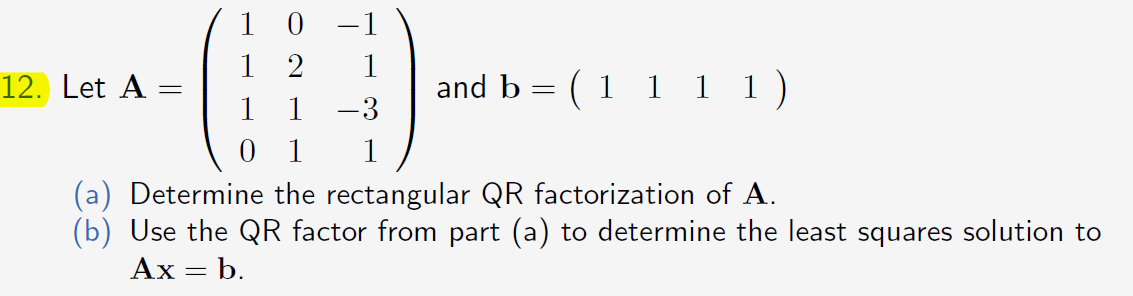
\includegraphics[scale=0.8]{question12.png}\\
(a)QR分解过程如下:
\begin{align*}
  k=1:\ \  
  &r_{11} \leftarrow ||a_1||=\sqrt{3}, \ \ \ \ \ \  
  q_1 \leftarrow \frac{a_1}{r_{11}} = \frac{1}{\sqrt{3}} 
  \left(
    \begin{matrix}
      1 \\ 1\\ 1\\ 0
    \end{matrix}
  \right) \\
  k=2: 
  &r_{12} \leftarrow q_1^Ta_2=\sqrt{3},\ \ \ \ \ \ 
  q_2\leftarrow a_2-r_{12}q_1 = a_2 - \sqrt{3}q_1 
  =\left(
    \begin{matrix}
      -1 \\ 1 \\ 0 \\ 1
    \end{matrix}
  \right), \\ 
  &r_{22} = ||q_2|| = \sqrt{3},\ \ \ \ \ \ 
  q_2 \leftarrow \frac{q_2}{r_{22}} = \frac{1}{\sqrt{3}}\left(
    \begin{matrix}
      -1 \\ 1 \\ 0 \\ 1
    \end{matrix}
  \right)\\
  k=3: 
  &r_{13} \leftarrow q_1^Ta_3=-\sqrt{3},\ \ \ \ \ \ 
  r_{23} \leftarrow q_2^Ta_3=\sqrt{3},\\ 
  &q_3\leftarrow a_3-r_{13}q_1 - r_{23}q_2 = a_3 + \sqrt{3}q_1 - \sqrt{3}q_2 
  =\left(
    \begin{matrix}
      1 \\ 1 \\ -2 \\ 0
    \end{matrix}
  \right), \\ 
  &r_{33} = ||q_3|| = \sqrt{6},\ \ \ \ \ \ 
  q_3 \leftarrow \frac{q_3}{r_{33}} = \frac{1}{\sqrt{6}}\left(
    \begin{matrix}
      1 \\ 1 \\ -2 \\ 0
    \end{matrix}
  \right)\\
\end{align*}

所以,可以得到,
\begin{align*}
  Q=\left(
  \begin{matrix}
    &\frac{\sqrt{3}}{3} & -\frac{\sqrt{3}}{3} &\frac{\sqrt{6}}{6}\\
    &\frac{\sqrt{3}}{3} & \frac{\sqrt{3}}{3} & \frac{\sqrt{6}}{6}\\
    &\frac{\sqrt{3}}{3} & 0 & -\frac{\sqrt{6}}{3}\\
    &0 & \frac{\sqrt{3}}{3} & 0
  \end{matrix}  
  \right), \ \ \ \ \ \ 
  R=\left(
    \begin{matrix}
      & \sqrt{3} & \sqrt{3} & -\sqrt{3} \\
      & 0 &\sqrt{3} & \sqrt{3} \\
      & 0 & 0 & \sqrt{6}
    \end{matrix}
  \right)
\end{align*}
(b)在上一题中已经求得A的QR分解形式$A=QR$,则等式$Ax=b$可以有如下形式
$$
Ax=b \Leftrightarrow QRx=b \Leftrightarrow Q^TQRx=Q^Tb \Leftrightarrow Rx=Q^Tb
$$
即
\begin{align*}
  \left(
    \begin{matrix}
      & \sqrt{3} & \sqrt{3} & -\sqrt{3} \\
      & 0 &\sqrt{3} & \sqrt{3} \\
      & 0 & 0 & \sqrt{6}
    \end{matrix}
  \right)
  \left(\begin{matrix}
    & x_1 \\
    & x_2 \\
    & x_3
  \end{matrix}
\right)
= \left(
  \begin{matrix}
    &\frac{\sqrt{3}}{3} & \frac{\sqrt{3}}{3} &\frac{\sqrt{3}}{3} & 0 \\
    &-\frac{\sqrt{3}}{3} & \frac{\sqrt{3}}{3} & 0 & \frac{\sqrt{3}}{3} \\
    &\frac{\sqrt{6}}{6} & \frac{\sqrt{6}}{6} & -\frac{\sqrt{6}}{3} & 0 \\
  \end{matrix}  
\right)
\left(\begin{matrix}
  & 1 \\
  & 1 \\
  & 1 \\
  & 1
\end{matrix}
\right)
=\left(
  \begin{matrix}
    & \sqrt{3} \\
    & \frac{\sqrt{3}}{3} \\
    & 0
  \end{matrix}  
\right)
\end{align*}
通过回代法可以求得
\begin{align*}
  x=\left(
    \begin{matrix}
      & \frac{2}{3} \\
      & \frac{1}{3} \\
      & 0
    \end{matrix}
  \right)
\end{align*}

\subsection*{Exercise.16}

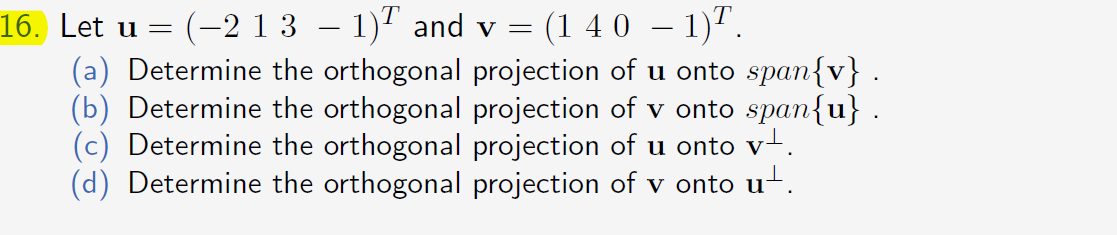
\includegraphics[scale=0.8]{question16.png}\\
(a)由于$v=(1\ \ 4 \ \ 0 \ \ -1)^T$,则
\begin{align*}
  P_v = \frac{vv^*}{v^*v}= 
  \frac{1}{18}
  \left(
    \begin{matrix}
      &1 &4 &0 &-1 \\
      &4 &16 &0 &-4 \\
      &0 &0 &0 &0 \\
      &-1 &-4 &0 &1 \\
    \end{matrix}
  \right)
\end{align*}
因此,$u$在$v$张成空间上的正交投影为
\begin{align*}
    P_vu=\frac{1}{18}
    \left(
      \begin{matrix}
        &1 &4 &0 &-1 \\
        &4 &16 &0 &-4 \\
        &0 &0 &0 &0 \\
        &-1 &-4 &0 &1 \\
      \end{matrix}
    \right)
    \left(
      \begin{matrix}
        &-2 \\
        &1 \\
        &3 \\
        &-1 \\
      \end{matrix}
    \right)
    =\frac{1}{6}\left(
      \begin{matrix}
        &1 \\
        &4 \\
        &0 \\
        &-1 \\
      \end{matrix}
    \right)
\end{align*}
(b)由于$u=(-2\ \ 1 \ \ 3 \ \ -1)^T$,则
\begin{align*}
  P_u = \frac{uu^*}{u^*u}= 
  \frac{1}{15}
  \left(
    \begin{matrix}
      &4 &-2 &-6 &2 \\
      &-2 &1 &3 &-1 \\
      &-6 &3 &9 &-3 \\
      &2 &-1 &-3 &1 
    \end{matrix}
  \right)
\end{align*}
因此,$v$在$u$张成空间上的正交投影为
\begin{align*}
    P_uv=\frac{1}{15}
    \left(
      \begin{matrix}
        &4 &-2 &-6 &2 \\
        &-2 &1 &3 &-1 \\
        &-6 &3 &9 &-3 \\
        &2 &-1 &-3 &1 
      \end{matrix}
    \right)
    \left(
      \begin{matrix}
        &1 \\
        &4 \\
        &0 \\
        &-1 \\
      \end{matrix}
    \right)
    =\frac{1}{5}\left(
      \begin{matrix}
        &-2 \\
        &1 \\
        &3 \\
        &-1 \\
      \end{matrix}
    \right)
\end{align*}
(c)由于$v=(1\ \ 4 \ \ 0 \ \ -1)^T$,则
\begin{align*}
  P_{v^\perp} =I - \frac{vv^*}{v^*v}= I-
  \frac{1}{18}
  \left(
    \begin{matrix}
      &1 &4 &0 &-1 \\
      &4 &16 &0 &-4 \\
      &0 &0 &0 &0 \\
      &-1 &-4 &0 &1 \\
    \end{matrix}
  \right)
  =\frac{1}{18}
  \left(
    \begin{matrix}
      &17 &-4 &0 &1 \\
      &-4 &2 &0 &4 \\
      &0 &0 &18 &0 \\
      &1 &4 &0 &17 
    \end{matrix}
  \right)
\end{align*}
因此,$u$在$v^\perp$张成空间上的正交投影为
\begin{align*}
    P_{v^\perp}u=\frac{1}{18}
    \left(
      \begin{matrix}
        &17 &-4 &0 &1 \\
        &-4 &2 &0 &4 \\
        &0 &0 &18 &0 \\
        &1 &4 &0 &17 
      \end{matrix}
    \right)
    \left(
      \begin{matrix}
        &-2 \\
        &1 \\
        &3 \\
        &-1 \\
      \end{matrix}
    \right)
    =\left(
      \begin{matrix}
        &-\frac{13}{6} \\
        &\frac{1}{3} \\
        &3 \\
        &-\frac{5}{6} \\
      \end{matrix}
    \right)
\end{align*}
(d)由于$u=(-2\ \ 1 \ \ 3 \ \ -1)^T$,则
\begin{align*}
  P_{u^\perp} =I - \frac{uu^*}{u^*u}
  = I - \frac{1}{15}
  \left(
    \begin{matrix}
      &11 &2 &6 &-2 \\
      &2 &14 &-3 &1 \\
      &6 &-3 &6 &3 \\
      &-2 &1 &3 &14 
    \end{matrix}
  \right)
\end{align*}
因此,$v$在$u^\perp$张成空间上的正交投影为
\begin{align*}
    P_{u^\perp}v=\frac{1}{15}
    \left(
      \begin{matrix}
        &11 &2 &6 &-2 \\
      &2 &14 &-3 &1 \\
      &6 &-3 &6 &3 \\
      &-2 &1 &3 &14 
      \end{matrix}
    \right)
    \left(
      \begin{matrix}
        &1 \\
        &4 \\
        &0 \\
        &-1 \\
      \end{matrix}
    \right)
    =\frac{1}{5}\left(
      \begin{matrix}
        &7 \\
        &19 \\
        &-3 \\
        &-4 \\
      \end{matrix}
    \right)
\end{align*}
\end{document}
